\subsection*{Teil D: Anwendungsaufgaben (20 Minuten)}
\textit{(Kombination aller Themenbereiche)}

\begin{enumerate}[label=\arabic*., resume]

    \item \textbf{Geometrie und Terme:}

    Ein Rechteck hat die Seitenlängen $(x + 3)$ cm und $(2x - 1)$ cm.

    \vspace{0.5cm}

    \begin{center}
        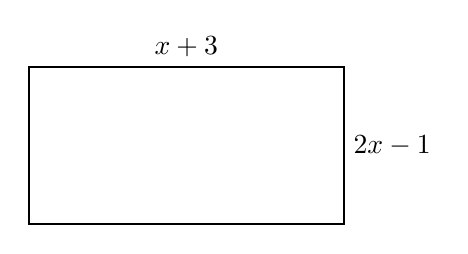
\begin{tikzpicture}[scale=1]
            \draw[thick] (0,0) rectangle (4,2);
            \node[above] at (2,2) {$x + 3$};
            \node[right] at (4,1) {$2x - 1$};
        \end{tikzpicture}
    \end{center}

    \begin{enumerate}[label=\alph*)]
        \item Stelle einen Term für den Umfang auf:

        \vspace{0.3cm}
        $U = 2 \cdot (x + 3) + 2 \cdot (2x - 1) = $ \underline{\hspace{4cm}}

        \vspace{0.5cm}

        \item Der Umfang beträgt 32 cm. Bestimme x:

        \vspace{0.3cm}
        Gleichung: \underline{\hspace{3cm}} $= 32$
        \vspace{0.3cm}
        Lösung: $x = $ \underline{\hspace{2cm}}

        \vspace{0.5cm}

        \item Wie lang sind die Seiten tatsächlich?

        \vspace{0.3cm}
        Länge: $(x + 3) = \phantom{0} + 3 = $ \underline{\hspace{2cm}} cm
        \vspace{0.3cm}
        Breite: $(2x - 1) = 2 \cdot \phantom{0} - 1 = $ \underline{\hspace{2cm}} cm

    \end{enumerate}

    \vspace{1cm}

    \item \textbf{Prozente und Gleichungen:}

    In einem Elektronikgeschäft kostet ein Tablet ursprünglich $x$ Euro. Nach einem Rabatt von 15\% kostet es 255 Euro.

    \vspace{0.5cm}

    \begin{enumerate}[label=\alph*)]
        \item Stelle eine Gleichung auf:

        \vspace{0.3cm}
        \textit{Überlegung:} 255 Euro entsprechen 85\% des ursprünglichen Preises.
        \vspace{0.3cm}
        Gleichung: $\dfrac{85 \cdot x}{100} = $ \underline{\hspace{2cm}}

        \vspace{0.5cm}

        \item Löse die Gleichung:

        \vspace{0.3cm}
        $85x = 255 \cdot \phantom{000}$
        \vspace{0.3cm}
        $x = $ \underline{\hspace{2cm}} Euro

        \vspace{0.5cm}

        \item Wie hoch war der Rabatt in Euro?

        \vspace{0.3cm}
        Rabatt = \underline{\hspace{2cm}} $- 255 = $ \underline{\hspace{2cm}} Euro

    \end{enumerate}

    \vspace{1cm}

    \item \textbf{Komplexe Anwendung:}

    Ein quadratisches Grundstück hat die Seitenlänge $(x + 4)$ Meter. Das Grundstück wird um einen 2 Meter breiten Streifen an allen Seiten vergrößert.

    \vspace{0.5cm}

    \begin{center}
        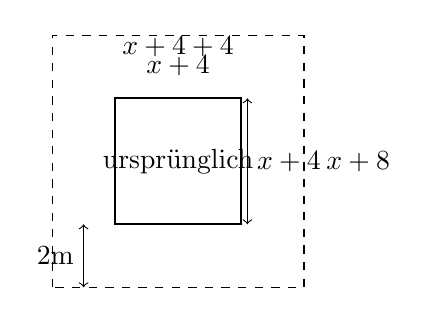
\begin{tikzpicture}[scale=0.8]
            % Inneres Quadrat
            \draw[thick] (1,1) rectangle (3,3);
            \draw[dashed] (0,0) rectangle (4,4);

            % Beschriftungen
            \node at (2,2) {ursprünglich};
            \node[above] at (2,3.5) {$x + 4 + 4$};
            \node[right] at (4.2,2) {$x + 8$};
            \node[above] at (2,3.2) {$x + 4$};

            % Streifen markieren
            \draw[<->] (3.1,1) -- (3.1,3);
            \node[right] at (3.1,2) {$x+4$};
            \draw[<->] (0.5,0) -- (0.5,1);
            \node[left] at (0.5,0.5) {2m};
        \end{tikzpicture}
    \end{center}

    \begin{enumerate}[label=\alph*)]
        \item Wie lang ist eine Seite des vergrößerten Grundstücks?

        \vspace{0.3cm}
        Seitenlänge = $(x + 4) + 2 + 2 = $ \underline{\hspace{3cm}} m

        \vspace{0.5cm}

        \item Stelle einen Term für die Fläche des vergrößerten Grundstücks auf:

        \vspace{0.3cm}
        $A = (x + 8)^2 = $ \underline{\hspace{4cm}} m²

        \vspace{0.5cm}

        \item Die Fläche des vergrößerten Grundstücks beträgt 144 m². Bestimme x:

        \vspace{0.3cm}
        $(x + 8)^2 = 144$
        \vspace{0.3cm}
        $x + 8 = 12$ \quad (da $12^2 = 144$)
        \vspace{0.3cm}
        $x = $ \underline{\hspace{2cm}} m

    \end{enumerate}

\end{enumerate}